\documentclass[a4paper, 12pt]{report}
\usepackage[utf8]{inputenc}
\usepackage[boxed,linesnumbered]{algorithm2e}
\usepackage[bookmarks, breaklinks, colorlinks]{hyperref}

\hypersetup{
	citecolor=black,
	linkcolor=black,
	filecolor=black,
	urlcolor=black
}

\usepackage{graphicx}
\usepackage{pdfpages}
\usepackage{tocbibind}
\usepackage{longtable}
\usepackage{array}
\usepackage{amsmath}

% FP table
\newenvironment{fptable}[2]{
	\begin{center}
	#1
	\begin{longtable}{|c|c|c|c|}
	\hline 
	&
	\multicolumn{3}{|c|}{{#2}}\\\nopagebreak\hline	
}{
	\hline\end{longtable}\end{center}
}

\newcommand{\fpvalues}[4]{%
	\textit{#1} & \textit{#2}& \textit{#3}& \textit{#4}\\\nopagebreak\hline
}

% FP count table
\newenvironment{fpcounttable}[1]{
	\begin{center}
	\begin{longtable}{|l|l|l|}
	\hline 
	#1 & Complexity & FPs \\\hline
}{
	\end{longtable}\end{center}
}

\newenvironment{fptotaltable}{
	\begin{center}
	\begin{longtable}{|l|r|}
	\hline 
	Function Type & Value \\\hline
}{
	\end{longtable}\end{center}
}

\newcommand{\fptotal}[1]{
	\multicolumn{2}{|l|}{{Total}}
	& #1\\\hline
}
\usepackage{listings}
\lstset{ %
  backgroundcolor=\color{white},   % choose the background color; you must add \usepackage{color} or \usepackage{xcolor}
  basicstyle=\footnotesize,        % the size of the fonts that are used for the code
  breakatwhitespace=false,         % sets if automatic breaks should only happen at whitespace
  breaklines=true,                 % sets automatic line breaking
  captionpos=b,                    % sets the caption-position to bottom
  commentstyle=\color{mygreen},    % comment style
  deletekeywords={...},            % if you want to delete keywords from the given language
  escapeinside={\%*}{*)},          % if you want to add LaTeX within your code
  extendedchars=true,              % lets you use non-ASCII characters; for 8-bits encodings only, does not work with UTF-8
  frame=single,	                   % adds a frame around the code
  keepspaces=true,                 % keeps spaces in text, useful for keeping indentation of code (possibly needs columns=flexible)
  keywordstyle=\color{blue},       % keyword style
  language=Java,                 % the language of the code
  %otherkeywords={*,...},           % if you want to add more keywords to the set
  numbers=left,                    % where to put the line-numbers; possible values are (none, left, right)
  numbersep=5pt,                   % how far the line-numbers are from the code
  numberstyle=\tiny\color{mygray}, % the style that is used for the line-numbers
  rulecolor=\color{black},         % if not set, the frame-color may be changed on line-breaks within not-black text (e.g. comments (green here))
  showspaces=false,                % show spaces everywhere adding particular underscores; it overrides 'showstringspaces'
  showstringspaces=false,          % underline spaces within strings only
  showtabs=false,                  % show tabs within strings adding particular underscores
  stepnumber=2,                    % the step between two line-numbers. If it's 1, each line will be numbered
  stringstyle=\color{mymauve},     % string literal style
  tabsize=2,	                   % sets default tabsize to 2 spaces
  %title=\lstname                   % show the filename of files included with \lstinputlisting; also try caption instead of title
  morecomment=[s]{/*}{*/},%
  morecomment=[l]//,
}

\def\chapterautorefname{Chapter}


\title{
	\begin{figure}[h]
		\centering
		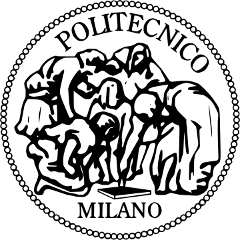
\includegraphics{../common_resources/logo_polimi.png}
	\end{figure}
	\vspace{30px}
	Software Engineering 2 Project: PowerEnJoy \\ \vspace{1em}
	\textbf{P}roject \textbf{P}lan
}
	

\author{Marco Ieni, Francesco Lamonaca, Marco Miglionico\\Politecnico di Milano, A.A. 2016/2017}
\date{\today\\v1.0}

\begin{document}
\maketitle
\tableofcontents
% \listoffigures
% \listoftables
\chapter{Introduction}
This is the project plan document for the PowerEnJoy project. In this document we will provide an estimate of the complexity of the project and an initial schedule of the work. In the second chapter we will evaluate the functions points, used in chapter three to estimate the cost and effort needed to develop PowerEnJoy, using COCOMO II. In chapter four we will provide an initial work schedule for the project and in chapter five an initial subdivision of the tasks among all the three components of the group. Finally in chapter six we will estimate which risks the project could incur in and how we think to avoid them. 


\chapter{Function Points Estimation}
\label{ch:function_points_estimation}
In this chapter we provide a comprehensive view over the system components, both at a physical and logical level.
The system will be firstly described at a very high level, showing the different components and how they interact (section 2.1).
Then the system will be described and detailed in the section 2.2, following a top-down approach.

In section 2.3 we will focus our attention more on the physical level, analysing the deployment of the system on physical tiers, while in section 2.4 we will describe the dynamic behaviour of the system.

Furthermore, section 2.5 will focus on the interface between the different components of the system.
Finally, the design choices and patterns used will be presented and discussed in section 2.6.

\section{Internal Logic Files (ILFs)}


\section{External Logic Files (ELFs)}
\section{External Inputs (EIs)}
External Inputs (EI) represent an elementary process in which data come from the external environment (like a data input screen or another application).

Our system involves many kind of interactions with different categories of inputs.
We are now going to summarize the impact of the offered features, grouping them by user category.

\begin{description}
	\item[Non registered user:] A Non Registered User is someone who has not been logged yet to the system. They can send inputs to the system mainly through these methods: 
	\begin{itemize}
	\item \textbf{Login/Logout}: the most complex part of these operation is the management of the password field in a secure way. Overall they contribute 4 FP each.
	\item \textbf{Registration:} We have to register all the fields provided by the user and to validate the document information. In addition to this we have to send a password to the user if the registration is successful. It contributes 9 FP.
	\end{itemize}
	
	\item[User:] A user is someone who has been logged to the system. They can send inputs to the system mainly through these methods: 
	\begin{itemize}
	\item\textbf{Edit profile data:} This is a trivial operation, because we have only to update the elements in the database, except for the editing of the password and the document information, that has to be validated again. It contributes 4 FP.
	\item\textbf{Delete account:} It contributes 2 FP.
	\item\textbf{Look for a car with user position or with a specified address:} These are both very complex operations, that involve a large number of components. For this reason they account for 18 FP in total.
	\item\textbf{Reserve and unlock a car:} These a trivial operation, because they require only to change the state of the car. They contribute 2 FP each.
	\item\textbf{Start the car:} The server has to check if the password that the user inserts in the tablet is correct and then it has to change the state of the car. It contributes 4 FP.
	\item\textbf{Know the current fee:} a user looks at the tablet of the car and reads the current fee. He or she can do this in every moment when he or she is in the vehicle, because the current fee is always displayed.
	\item\textbf{Enable saving money option:} This is an operation with high complexity, because the system has to compute the best station where to leave the car. It accounts for 18 FP.
	\end{itemize}
	
	\item[HandyCar Board:] The board installed on every car of PowerEnjoy. It can send inputs to the system mainly through these methods: 
	\begin{itemize}
	\item\textbf{End the ride:} When the car is parked in a safe area and the user exits the car the HandyCar Board signal this event to the system. It has a very low complexity, so it contributes 1 FP.
	\item\textbf{Car recharged:} The user connects the car to a plug of a power grid station, so the HandyCar Board signal this event to the system. It has a very low complexity, so it contributes 1 FP.
	\end{itemize}
	
	\item[Operator:] The PowerEnjoy employees that has to manage the system from an high level point of view. They can send inputs to the system mainly through these methods: 
	\begin{itemize}
	\item\textbf{Add a Safe Area:} After some consistency check, the system has to update the database simply adding the new safe area. It has a very low complexity, so it contributes 1 FP.
	\item\textbf{Delete a Safe Area:} After some consistency check, the system has to update the database and wait enough time to avoid creating inconvenience to the user that are using that safe area. It contributes 4 FP.
	\item\textbf{Add a Power Grid Station:} After some consistency check, the system has to update the database simply adding the new power grid station. It has a very low complexity, so it contributes 1 FP.
	\item\textbf{Delete a Power Grid Station:} After some consistency check, the system has to update the database by eliminating that power grid station. It contributes 1 FP.
	\end{itemize}
	
\end{description}
\section{External Inquiries (EQs)}
External Inquiry (EQ) represents an elementary process with both input and output components that result in data retrieval from one or more internal logical files and external interface files.
There must be no significant elaboration of data from logic files.

Our system supports the following EQs:
\begin{itemize}
	\item Consulting history of the rides;
	\item Get info about a given car identified by its plate, like the model, the number of passengers and so on;
	\item Retrieve the list of all the safe areas;
	\item Retrieve the list of all the power grid stations;
	\item Retrieve the actual values of the sensors and actuators of a given car;
\end{itemize}

The resulting table is the following:

\begin{fpcounttable}{EQ}
Consult ride history & Low & 2 \\
Get car info & Low & 2 \\
Retrieve list of safe areas & Low & 2 \\
Retrieve list of power grid stations & Low & 2 \\
Retrieve car sensors and actuators & Low & 2 \\\hline 
\fptotal{10}	
\end{fpcounttable}
\section{External Outputs (EOs)}
\section{Overall estimation}
The following table summarizes the results of our estimation activity:

\begin{fptotaltable}
	Internal Logic Files & 64 \\
	External Logic Files & 22 \\
	External Inputs & 77 \\
	External Inquiries & 10 \\
	External Outputs & 10 \\\hline
	Total & 183\\\hline
\end{fptotaltable}

Relying on the QSM Function Point Languages Table v5.0 and considering Java Enterprise Edition as a development platform, leaving the aspects related to the implementation of the mobile applications (which can be thought as pure presentation with no business logic), in the following we can estimate the total number of lines of code.

Average approximation:
\begin{lstlisting}[stepnumber=0]
	SLOC = 183 * 46 = 8418
\end{lstlisting}
Upper bound:
\begin{lstlisting}[stepnumber=0]
	SLOC = 183 * 67 = 12261	
\end{lstlisting}



\chapter{Cost and Effort Estimation}
\label{ch:cost_effor_estimation}
\section{Cost and effort estimation: COCOMO II}
In this section we are going to use the COCOMO II approach to estimate the
cost and effort needed to develop PowerEnJoy.
\subsection{Scale Drivers}
In order to evaluate the values of the scale drivers, we refer to the following
official COCOMO II table:

\begin{longtable}{| m{1,8 cm}| m{1,8 cm} | m{1,8 cm} | m{1,8 cm} | m{1,8 cm} | m{2,2 cm} | m{1,8 cm}| }
\hline
\textbf{Scale Factors} & \textbf{Very Low} & \textbf{Low} & \textbf{Nominal} & \textbf{High} & \textbf{Very High} & \textbf{Extra High}\\
\hline
PREC & thoroughly unprecedented & largely unprecedented & somewhat unprecedented & generally familiar & largely familiar & thoroughly familiar \\
\newline $SF_j$ & 6.20 & 4.96 & 3.72 & 2.48 & 1.24 & 0.00 \\
\hline
FLEX & rigorous & occasional relaxation & some relaxation & general conformity & some conformity & general goals \\
\newline $SF_j$ & 5.07 & 4.05 & 3.04 & 2.03 & 1.01 & 0.00 \\
\hline
RESL & little(20\%) & some(40\%) & often(60\%) & generally (75\%) & mostly(90\%) & full(100\%) \\
\newline $SF_j$ & 7.07 & 5.65 & 4.24 & 2.83 & 1.41 & 0.00 \\
\hline
TEAM & very difficult interactions & some difficult interactions & basically cooperative interactions & largely cooperative & highly cooperative & seamless interactions \\
\newline $SF_j$ & 5.48 & 4.38 & 3.29 & 2.19 & 1.10 & 0.00\\
\hline
PMAT & Level 1 Lower & Level 1 Upper & Level 2 & Level 3 & Level 4 & Level 5 \\
\newline $SF_j$ & 7.80 & 6.24 & 4.68 & 3.12 & 1.56 & 0.00\\
\hline
\end{longtable}

A brief description for each scale driver:
\begin{itemize}
\item\textbf{Precedentedness}:it reflects the previous experience of our team in the development of similar project. In our case, since we don't have this kind of experience the value will be low. 

\item\textbf{Development Flexibility}:it reflects the degree of flexibility in the development process with respect to the external specification and requirements.We set it to nominal because we have to follow a prescribed process, but we had a certain degree of flexibility in the definition of the requirements and in the design process.

\item\textbf{Architecture/Risk resolution}: it reflects the level of awareness and reactiveness with
respect to risks. The risk analysis we performed is quite extensive, so we have a clear definition of budget and schedule,for this reason the value will be set to very high.

\item\textbf{Team cohesion}: it reflects how well the development team know each other and work together. We set it to very high, since the cohesion among the three of us is optimal .

\item\textbf{Process maturity}: it reflects the process maturity of the organization. We set it to 3 because the  process comes very close to achieving the specific objectives such as quality, cost, and schedule. Besides processes, standards, procedures and tools were already defined
at the organizational level.
\end{itemize}

The estimated scale drivers for our project, together with the formula to
compute the exponent E are the following:
\begin{longtable}{| m{6 cm}| m{6 cm} | m{2 cm} |}
\hline
\textbf{Scale Drivers} & \textbf{Factor} & \textbf{Value} \\
\hline
Precedentedness(PREC) & Low & 4.96 \\
\hline
Development flexibility(FLEX) & Nominal & 3.04 \\
\hline
Risk Resolution(RESL) & Very High & 1.41 \\
\hline
Team Cohesion (TEAM) & Very High & 1.10 \\
\hline
Process Maturity (PMAT) & Level 3 & 3.12 \\
\hline
\textbf{Total} & & 13.63\\
\hline
\textbf{Total} & E=0.91 + 0.01 x $\sum_{1<=j<=5} SF_j$ & 1.0463 \\
\hline
\end{longtable}

\subsection{Cost Drivers}
Cost Drivers are the parameters of the Effort Equation that reflect some characteristics of the developing process and act as multiplicators on the effort needed to build the project. They appear as factors in the Effort Equation. Cost Drivers are described in detail in the COCOMO Manual [6, p. 25].
The cost drivers are the following:
\begin{itemize}
\item \textbf{Required Software Reliability}: Since this is not the only car sharing system in the city,an eventual malfunctioning could led to moderate financial losses,for this reason we set the RELY cost driver to nominal. 

\begin{longtable}{| m{1,8 cm}| m{1,8 cm} | m{1,8 cm} | m{1,8 cm} | m{1,8 cm} | m{1,8 cm} | m{1,8 cm}| }
\hline
\multicolumn{7}{c}{RELY Cost Drivers}\\
\hline
\hline
RELY Descriptors & slightly inconvenience & easy recoverable losses & moderate recoverable losses & high financial losses & risk to human life & \\
\hline
Rating level & very low & low & nominal & high & very high & extra high \\
\hline
Effort multipliers & 0.82 & 0.92 & 1.00 & 1.10 & 1.26 & n/a \\
\hline
\end{longtable}

\item \textbf{Database size}: This measure considers the effective size of our database. We don't have the exact size, but our estimation given the tables and fields we have is to reach a 1GB database. Since it is
distributed over??????? 10.000-15.000 SLOC, the ratio D/P (measured as testing DB bytes/program SLOC) is between 209 and 314 resulting in the DATA cost driver being nominal.\\ \\ \\ %TODO 10.000-15.000 SLOC, the ratio D/P (measured as testing DB bytes/program SLOC) is between 209 and 314 

\begin{longtable}{| m{1,5 cm}| m{1,5 cm} | m{1,5 cm} | m{2,4 cm} | m{2,6 cm} | m{1,5 cm} | m{1,5 cm}| }
\hline
\multicolumn{7}{c}{DATA Cost Drivers}\\
\hline
\hline
DATA Descriptors &  & \begin{equation*}
 {D \over P} {<10} 
\end{equation*} & 
\begin{equation*}
{10\le} {D \over P} {\le 100}
\end{equation*}& 
\begin{equation*}
{100\le} {D \over P} {\le 1000}
\end{equation*} & 
\begin{equation*}
 {D \over P} {>1000} 
\end{equation*}
& \\
\hline
Rating level & very low & low & nominal & high & very high & extra high \\
\hline
Effort multipliers & 0.82 & 0.92 & 1.00 & 1.10 & 1.26 & n/a \\
\hline
\end{longtable}

\item \textbf{Product Complexity}:
Set to high according to the COCOMO II rating scale.

\begin{longtable}{| m{1,8 cm}| m{1,8 cm} | m{1,8 cm} | m{1,8 cm} | m{1,8 cm} | m{1,8 cm} | m{1,8 cm}| }
\hline
\multicolumn{7}{c}{CPLX Cost Drivers}\\
\hline
\hline
Rating level & very low & low & nominal & high & very high & extra high \\
\hline
Effort multipliers & 0.73 & 0.87 & 1.00 & 1.17 & 1.34 & 1.74 \\
\hline
\end{longtable}

\item \textbf{Required Re-usability}:
In our case, the re-usability requirements are just across projects, so the RUSE cost driver is set to nominal.

\begin{longtable}{| m{1,8 cm}| m{1,8 cm} | m{1,8 cm} | m{1,8 cm} | m{1,8 cm} | m{1,8 cm} | m{1,8 cm}| }
\hline
\multicolumn{7}{c}{RUSE Cost Drivers}\\
\hline
\hline
RUSE Descriptors &  & None & Across projects & Across programs & Across product line & Across multiple product line\\
\hline
Rating level & very low & low & nominal & high & very high & extra high \\
\hline
Effort multipliers & n/a & 0.95 & 1.00 & 1.07 & 1.15 & 1.24 \\
\hline
\end{longtable}

\item \textbf{Documentation match to life-cycle needs}:This parameter is evaluated in terms of the suitability of the project's documentation to its life-cycle needs. In our case, every need
of the product life-cycle is already present in the documentation,
so the DOCU cost driver is set to nominal.

\begin{longtable}{| m{1,8 cm}| m{1,8 cm} | m{1,8 cm} | m{1,8 cm} | m{1,8 cm} | m{1,8 cm} | m{1,8 cm}| }
\hline
\multicolumn{7}{c}{DOCU Cost Drivers}\\
\hline
\hline
DOCU Descriptors & Many life-cycle needs uncovered & Some life-cycle needs uncovered & Right-sized to life-cycle needs & Excessive for life-cycle needs & Very excessive for life-cycle needs & \\
\hline
Rating level & very low & low & nominal & high & very high & extra high \\
\hline
Effort multipliers & 0.81 & 0.91 & 1.00 & 1.11 & 1.23 & n/a \\
\hline
\end{longtable}

\item \textbf{Execution time constraint}:This parameter is a measure of the CPU usage imposed upon a software system. The rating is expressed in terms of the percentage of available execution time expected to be used by the system or subsystem consuming the execution time resource. In our case,since the software is quite complex,our our expectancy is that its CPU usage will be high.

\begin{longtable}{| m{1,8 cm}| m{1,8 cm} | m{1,8 cm} | m{1,8 cm} | m{1,8 cm} | m{1,8 cm} | m{1,8 cm}| }
\hline
\multicolumn{7}{c}{TIME Cost Drivers}\\
\hline
\hline
TIME Descriptors &  &  & \begin{equation*}
{\le 50\%} 
\end{equation*} use of available execution time & 70\% use of available execution time & 85\% use of available execution time & 95\% use of available execution time \\
\hline
Rating level & very low & low & nominal & high & very high & extra high \\
\hline
Effort multipliers & n/a & n/a & 1.00 & 1.11 & 1.29 & 1.63 \\
\hline
\end{longtable}

\item \textbf{Storage Constraint}: This parameter represents the degree of main storage constraint imposed on a software system or subsystem.As the modern disk drives can easily contain several terabytes of storage, this value is set to nominal.

\begin{longtable}{| m{1,8 cm}| m{1,8 cm} | m{1,8 cm} | m{1,8 cm} | m{1,8 cm} | m{1,8 cm} | m{1,8 cm}| }
\hline
\multicolumn{7}{c}{STOR Cost Drivers}\\
\hline
\hline
STOR Descriptors &  &  & \begin{equation*}
{\le 50\%} 
\end{equation*} use of available storage& 70\% use of available storage & 85\% use of available storage & 95\% use of available storage \\
\hline
Rating level & very low & low & nominal & high & very high & extra high \\
\hline
Effort multipliers & n/a & n/a & 1.00 & 1.05 & 1.17 & 1.46 \\
\hline
\end{longtable}

\item \textbf{Platform Volatility}:"Platform" is used here to mean the complex of hardware and software (OS, DBMS, etc.) the software product calls on to perform its tasks. In our case we don’t expect our fundamental platforms to change very often. However, the client applications may require at least a major release once every six months to be aligned with the development cycle of the main mobile operating systems. For this reason, this parameter is set to nominal.

\begin{longtable}{| m{1,8 cm}| m{1,8 cm} | m{1,8 cm} | m{1,8 cm} | m{1,8 cm} | m{1,8 cm} | m{1,8 cm}| }
\hline
\multicolumn{7}{c}{PVOL Cost Drivers}\\
\hline
\hline
PVOL Descriptors &  & Major change every 12 mo;minor change every 1 & Major change every 6mo;minor change every 2wk & Major change every 2mo;minor change every 1wk & Major change every 2wk;minor change every 2 days & \\
\hline
Rating level & very low & low & nominal & high & very high & extra high \\
\hline
Effort multipliers & n/a & 0.87 & 1.00 & 1.15 & 1.30 & n/a \\
\hline
\end{longtable}

\item\textbf{Analyst Capability}:Analysts are personnel that work on requirements, high level design and detailed design. The major attributes that should be considered in this rating are Analysis and Design ability, efficiency and thoroughness, and the ability to communicate and cooperate.We think the analysis of the problem has been conducted in very precise and complete way with respect to a potential real world
implementation. For this reason, this parameter is set to high.

\begin{longtable}{| m{1,8 cm}| m{1,8 cm} | m{1,8 cm} | m{1,8 cm} | m{1,8 cm} | m{1,8 cm} | m{1,8 cm}| }
\hline
\multicolumn{7}{c}{ACAP Cost Drivers}\\
\hline
\hline
ACAP Descriptors & 15th percentile  & 35th percentile & 55th percentile & 75th percentile & 90th percentile & \\
\hline
Rating level & very low & low & nominal & high & very high & extra high \\
\hline
Effort multipliers & 1.42 & 1.19 & 1.00 & 0.85 & 0.71 & n/a \\
\hline
\end{longtable}

\item \textbf{Programmer Capability}:Evaluation should be based on the capability of the programmers as a team rather than as individuals. Major factors which should be considered in the rating are ability, efficiency and thoroughness, and the ability to communicate and cooperate. The experience of the programmer should not be considered here; it is rated with AEXP.We have not implemented the project, so this parameter is just an estimation; however we think our programming ability are good,but the most important thing is that we know each other and the level of communication and cooperation is optimal, for this reason we set this parameter to high.

\begin{longtable}{| m{1,8 cm}| m{1,8 cm} | m{1,8 cm} | m{1,8 cm} | m{1,8 cm} | m{1,8 cm} | m{1,8 cm}| }
\hline
\multicolumn{7}{c}{PCAP Cost Drivers}\\
\hline
\hline
PCAP Descriptors & 15th percentile  & 35th percentile & 55th percentile & 75th percentile & 90th percentile & \\
\hline
Rating level & very low & low & nominal & high & very high & extra high \\
\hline
Effort multipliers & 1.34 & 1.15 & 1.00 & 0.88 & 0.76 & n/a \\
\hline
\end{longtable}

\item\textbf{Application Experience}:This rating is dependent on the level of applications experience of the project team developing the software system or subsystem. We have some experience in the development of Java applications,in particular we made just one project of considerable size,for this reason and for the fact that we never had experience with Java EE we set this parameter to low.

\begin{longtable}{| m{1,8 cm}| m{1,8 cm} | m{1,8 cm} | m{1,8 cm} | m{1,8 cm} | m{1,8 cm} | m{1,8 cm}| }
\hline
\multicolumn{7}{c}{APEX Cost Drivers}\\
\hline
\hline
APEX Descriptors & \begin{equation*}
{\le 2}
\end{equation*} months  & 6 months & 1 year & 3 years & 6 years & \\
\hline
Rating level & very low & low & nominal & high & very high & extra high \\
\hline
Effort multipliers & 1.22 & 1.10 & 1.00 & 0.88 & 0.81 & n/a \\
\hline
\end{longtable}

\item \textbf{Platform Experience}:
As we said before we don’t have any experience with the Java EE platform, but
we have some previous experience with databases, user interfaces
and server side development. For this reason, we set
this parameter to nominal.

\begin{longtable}{| m{1,8 cm}| m{1,8 cm} | m{1,8 cm} | m{1,8 cm} | m{1,8 cm} | m{1,8 cm} | m{1,8 cm}| }
\hline
\multicolumn{7}{c}{PLEX Cost Drivers}\\
\hline
\hline
PLEX Descriptors & \begin{equation*}
{\le 2}
\end{equation*} months  & 6 months & 1 year & 3 years & 6 years & \\
\hline
Rating level & very low & low & nominal & high & very high & extra high \\
\hline
Effort multipliers & 1.19 & 1.09 & 1.00 & 0.91 & 0.85 & n/a \\
\hline
\end{longtable}

\item\textbf{Language and Tool Experience}:This parameter measure the level of programming language and software tool experience of the project team developing the software system or subsystem. We don’t have any experience with the Java EE platform, but we have some previous experience with databases, user interfaces and server side development. We also know the development environment, so we’re going to set this parameter to nominal.

\begin{longtable}{| m{1,8 cm}| m{1,8 cm} | m{1,8 cm} | m{1,8 cm} | m{1,8 cm} | m{1,8 cm} | m{1,8 cm}| }
\hline
\multicolumn{7}{c}{LTEX Cost Drivers}\\
\hline
\hline
LTEX Descriptors & \begin{equation*}
{\le 2}
\end{equation*} months  & 6 months & 1 year & 3 years & 6 years & \\
\hline
Rating level & very low & low & nominal & high & very high & extra high \\
\hline
Effort multipliers & 1.20 & 1.09 & 1.00 & 0.91 & 0.84 & n/a \\
\hline

\item \textbf{Personnel continuity}:The rating scale for PCON is in terms of the project's annual personnel turnover. In our case since we have very strict deadlines and since the time we can
spend on this project is limited we set this parameter to very low.

\begin{longtable}{| m{1,8 cm}| m{1,8 cm} | m{1,8 cm} | m{1,8 cm} | m{1,8 cm} | m{1,8 cm} | m{1,8 cm}| }
\hline
\multicolumn{7}{c}{PCON Cost Drivers}\\
\hline
\hline
PCON Descriptors & 48\% / year & 24\% / year & 12\% / year & 6\% / year & 3\% / year & \\
\hline
Rating level & very low & low & nominal & high & very high & extra high \\
\hline
Effort multipliers & 1.29 & 1.12 & 1.00 & 0.90 & 0.81 & n/a \\
\hline
\end{longtable}

\textbf{Usage of Software Tools}: Our application environment is quite complete and well integrated, so
we set this parameter as nominal.

\begin{longtable}{| m{1,8 cm}| m{1,8 cm} | m{1,8 cm} | m{1,8 cm} | m{1,8 cm} | m{1,8 cm} | m{1,8 cm}| }
\hline
\multicolumn{7}{c}{TOOL Cost Drivers}\\
\hline
\hline
TOOL Descriptors & edit,code,debug & simple,frontend,backend CASE,little integration & basic life-cycle tools,moderately integrated & strong,mature life-cycle tools,moderately integrated & strong,mature, proactive life-cycle tools, well integrated with processes,methods,reuse
& \\
\hline
Rating level & very low & low & nominal & high & very high & extra high \\
\hline
Effort multipliers & 1.17 & 1.09 & 1.00 & 0.90 & 0.78 & n/a \\
\hline
\end{longtable}

\textbf{Multisite development}:Even if we live in different cities, we have met a considerable number of times and we have also collaborated hugely through Internet services including social networks,Skype,email
and Whatsapp. For this reason, we  set this parameter to very high.

\begin{longtable}{| m{1,8 cm}| m{1,8 cm} | m{1,8 cm} | m{1,8 cm} | m{1,8 cm} | m{1,8 cm} | m{1,8 cm}| }
\hline
\multicolumn{7}{c}{SITE Cost Drivers}\\
\hline
\hline
SITE Collocation Descriptors & International & Multi-city and multi-company & Multi-city or multi-company & Same building or complex  & Fully collocated \\
\hline
SITE Communication Descriptors & Some phone,email & Individual phone,fax & Narrow band email & Wideband electronic communication &  Wideband electronic comm. and occasionally video conf. & Interactive multimedia \\ 
Rating level & very low & low & nominal & high & very high & extra high \\
\hline
Effort multipliers & 1.22 & 1.09 & 1.00 & 0.93 & 0.86 & 0.80 \\
\hline
\end{longtable}













\end{itemize}
\subsection{Effort equation}
This final equation gives us the effort estimation measured in Person-Months (PM):
\begin{lstlisting}[mathescape, numbers=none]
	Effort = A * EAF * KSLOC$^E$
\end{lstlisting}
where:
\begin{lstlisting}[mathescape, numbers=none]
	A = 2.94 (for COCOMO II.2000) 
	EAF = product of all cost drivers (1.1855)
	E = exponent derived from the scale drivers. It is computed as:
		B + 0.01 * $\sum_{i} SF[i]$ = B + 0.01 * 13.63 = 0.91 + 0.1363 = 1.0463
		in which B is equal to: 0.91 for COCOMO II.
\end{lstlisting}

With this parameters we can compute the effort value, which has a lower bound of:
\begin{lstlisting}[mathescape, numbers=none]
	Effort = A * EAF * KSLOC$^E$ = 2.94 * 1.1855 * 8418$^{1.0463}$ = 44.586 PM $\approx$ 45 PM
\end{lstlisting}
and an upper bound of:
\begin{lstlisting}[mathescape, numbers=none]
	Effort = A * EAF * KSLOC$^E$ = 2.94 * 1.1855 * 12261$^{1.0463}$ = 66.081 PM $\approx$ 66 PM
\end{lstlisting}

\subsection{Schedule estimation}
Regarding the final schedule, we are going to use the following formula:
\begin{lstlisting}[mathescape, numbers=none]
	Duration = 3.67 * Effort$^F$
\end{lstlisting}
As a lower bound, we consider
\begin{lstlisting}[mathescape, numbers=none]
	F = 0.28 + 0.2 * (E - B) = 0.28 + 0.2 * 0.1363 = 0.30726
	Effort = 44.586 PM 
	Duration = 3.67 * (44.586)$^{0.30726}$ = 11.79 months
\end{lstlisting}
while as an upper bound, we consider
\begin{lstlisting}[mathescape, numbers=none]
	F = 0.28 + 0.2 * (E - B) = 0.28 + 0.2 * 0.1363 = 0.30726
	Effort = 66.081 PM 
	Duration = 3.67 * (66.081)$^{0.30726}$ = 13.30 months
\end{lstlisting}
which seem to be both reasonable estimates.

\chapter{Schedule}
In this chapter, we will provide a general project schedule. More refined schedule will be provided during project development, in order to reflect eventual changes. Even if this project is made only for didactic purpose we will provided a hypothetical schedule of the development phase of the project, that we will not deal with.  This is to mimic how a real project should work.
In order to maintain readability, we split the schedule into five parts: one for the RASD, one for the DD, one for the ITPS and PPD and two for the development.
\begin{figure}
	\centering
	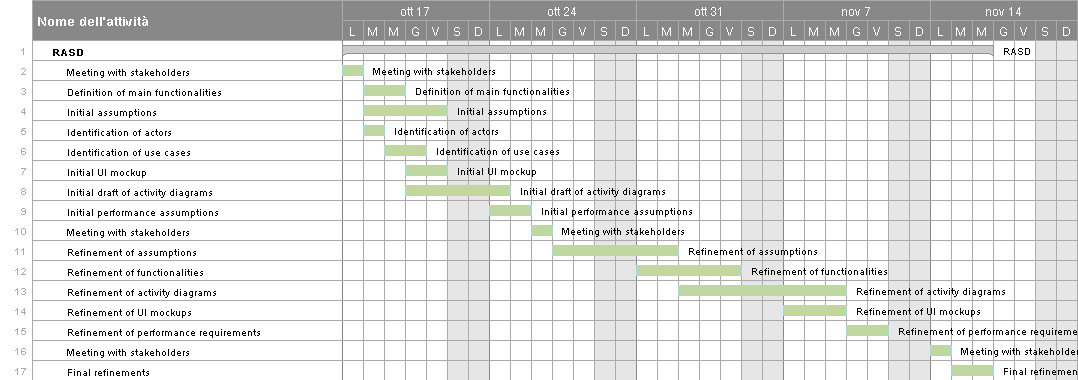
\includegraphics[width=\textwidth,height=\dimexpr\textheight-4\baselineskip-\abovecaptionskip-\belowcaptionskip\relax,keepaspectratio]{schedule/RASD.png}
\end{figure}
\begin{figure}
	\centering
	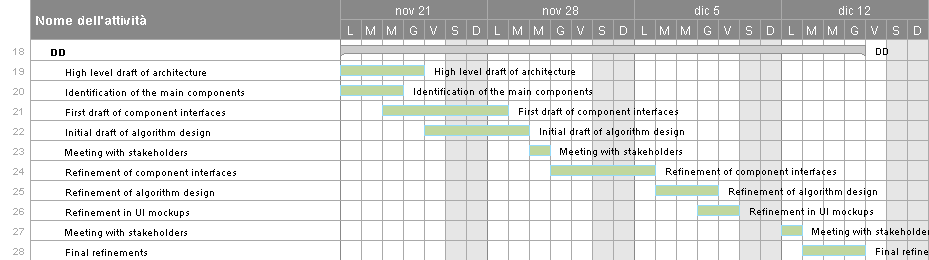
\includegraphics[width=\textwidth,height=\dimexpr\textheight-4\baselineskip-\abovecaptionskip-\belowcaptionskip\relax,keepaspectratio]{schedule/DD.png}
\end{figure}
\begin{figure}
	\centering
	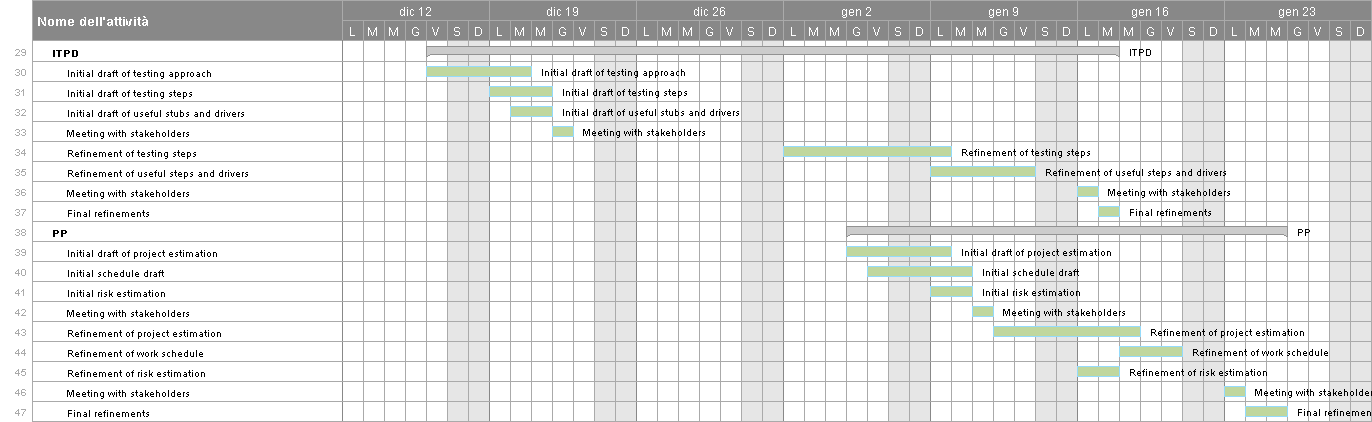
\includegraphics[width=\textwidth,height=\dimexpr\textheight-4\baselineskip-\abovecaptionskip-\belowcaptionskip\relax,keepaspectratio]{schedule/ITDP_PP.png}
\end{figure}
\begin{figure}
	\centering
	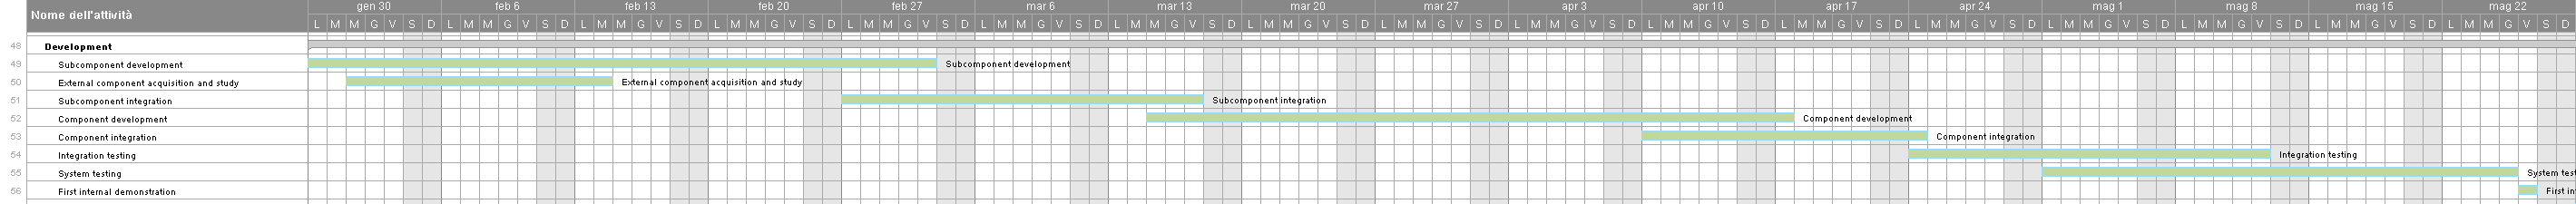
\includegraphics[width=\textwidth,height=\dimexpr\textheight-4\baselineskip-\abovecaptionskip-\belowcaptionskip\relax,keepaspectratio]{schedule/Develop1.png}
\end{figure}
\begin{figure}
	\centering
	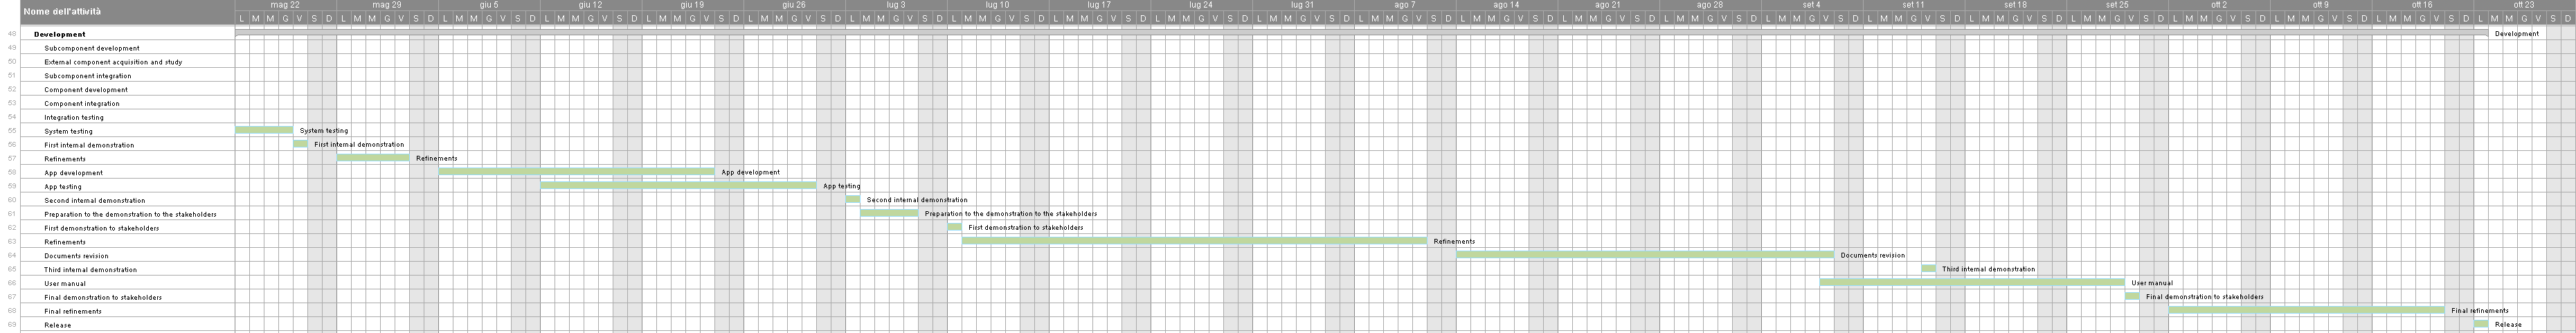
\includegraphics[width=\textwidth,height=\dimexpr\textheight-4\baselineskip-\abovecaptionskip-\belowcaptionskip\relax,keepaspectratio]{schedule/Develop2.png}
\end{figure}

\chapter{Resource Allocation}
In this chapter, we will describe how the tasks defined into the previous chapter will be divided between the three members of the group. As already mention we consider also the development phase of the project, and in order to maintain readability we split the schedule into five part.

\section{Marco Ieni}
\begin{center}
  \makebox[\textwidth]{
    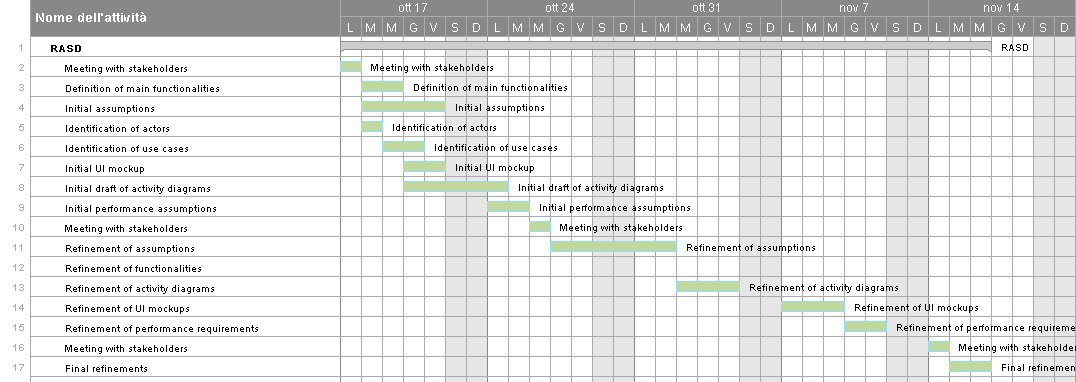
\includegraphics[width=\paperwidth]{resource_allocation/ieni/mi1.png}
	}
\end{center}

\begin{center}
  \makebox[\textwidth]{
    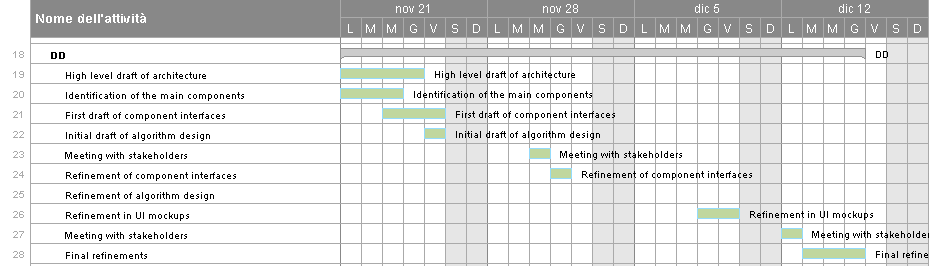
\includegraphics[width=\paperwidth]{resource_allocation/ieni/mi2.png}
	}
\end{center}

\begin{center}
  \makebox[\textwidth]{
    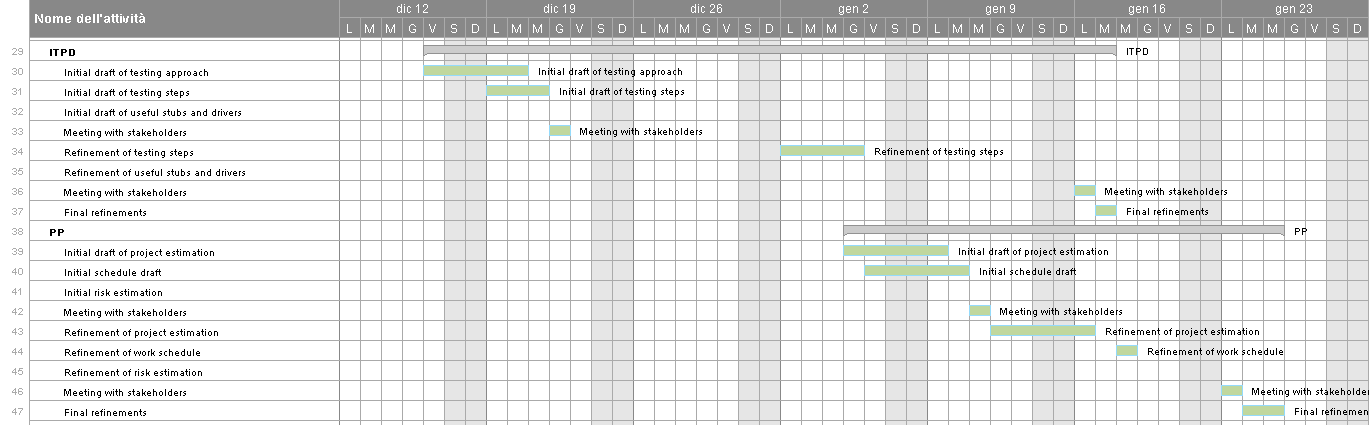
\includegraphics[width=\paperwidth]{resource_allocation/ieni/mi3.png}
	}
\end{center}

\begin{center}
  \makebox[\textwidth]{
    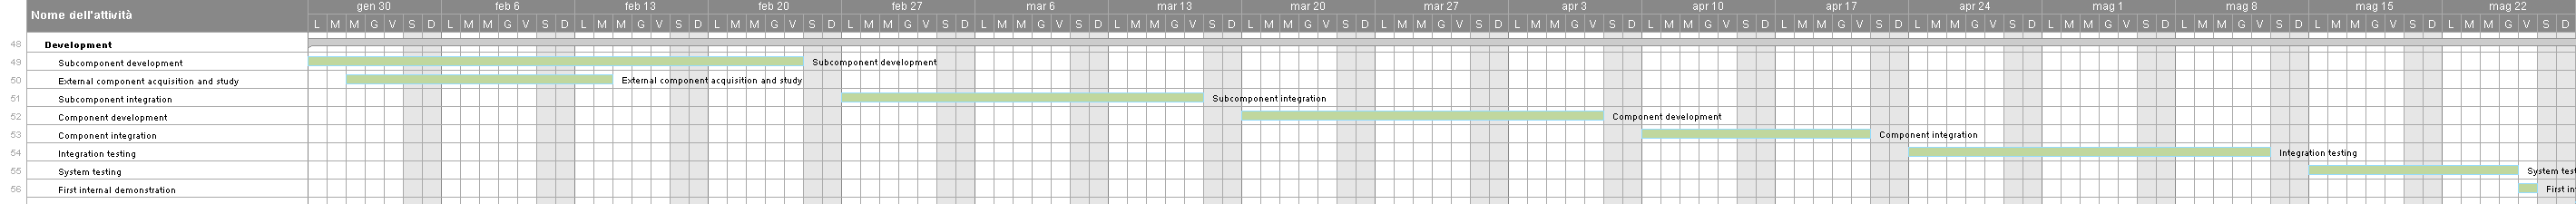
\includegraphics[width=\paperwidth]{resource_allocation/ieni/mi4.png}
	}
\end{center}

\begin{center}
  \makebox[\textwidth]{
    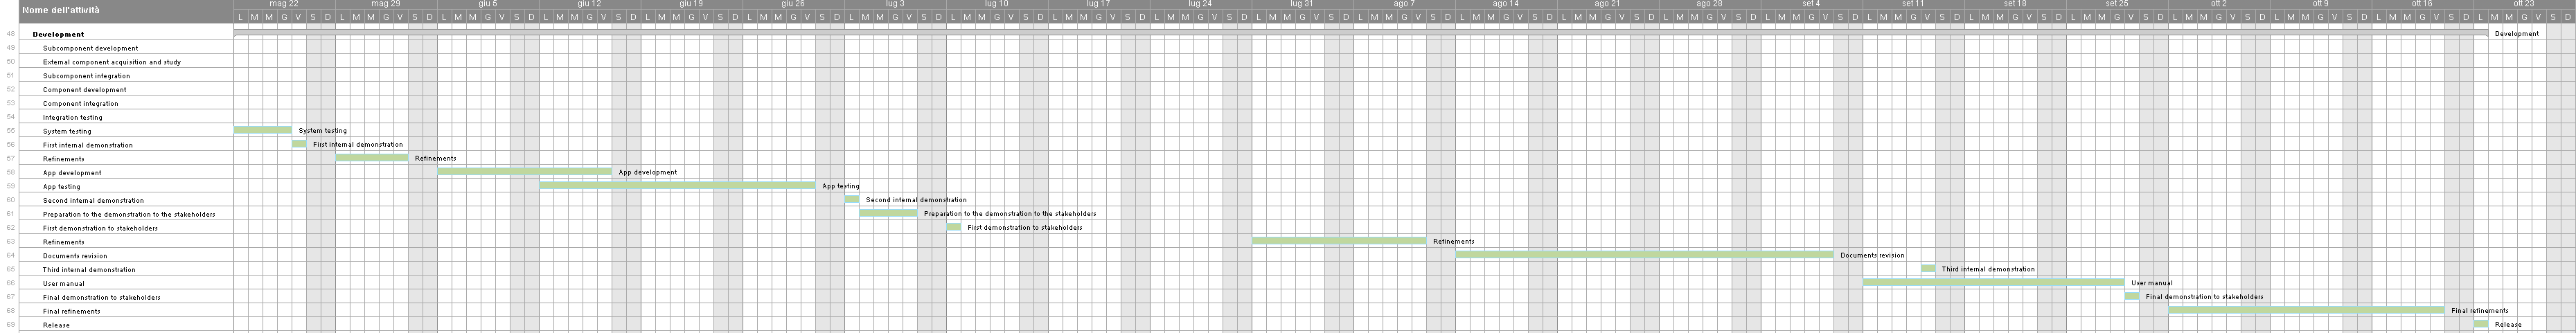
\includegraphics[width=\paperwidth]{resource_allocation/ieni/mi5.png}
	}
\end{center}


\section{Francesco Lamonaca}

\begin{center}
  \makebox[\textwidth]{
    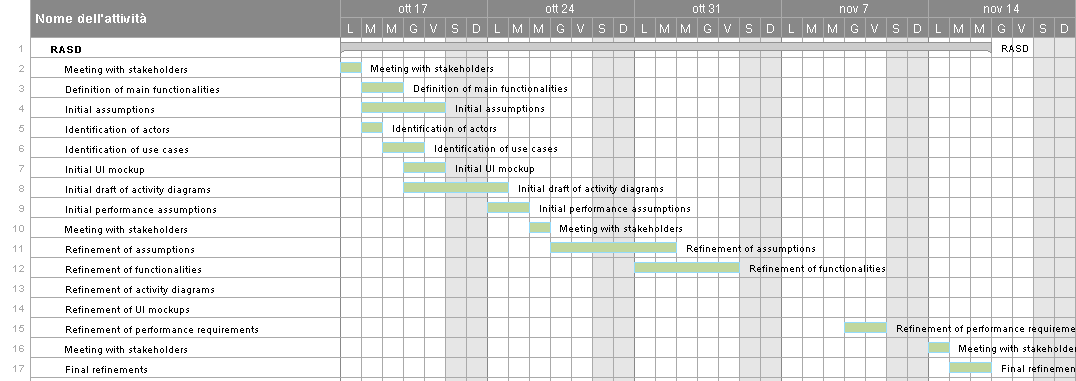
\includegraphics[width=\paperwidth]{resource_allocation/lamonaca/fl1.png}
	}
\end{center}

\begin{center}
  \makebox[\textwidth]{
    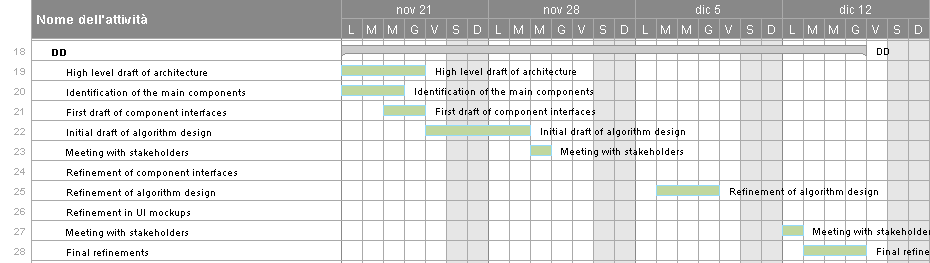
\includegraphics[width=\paperwidth]{resource_allocation/lamonaca/fl2.png}
	}
\end{center}

\begin{center}
  \makebox[\textwidth]{
    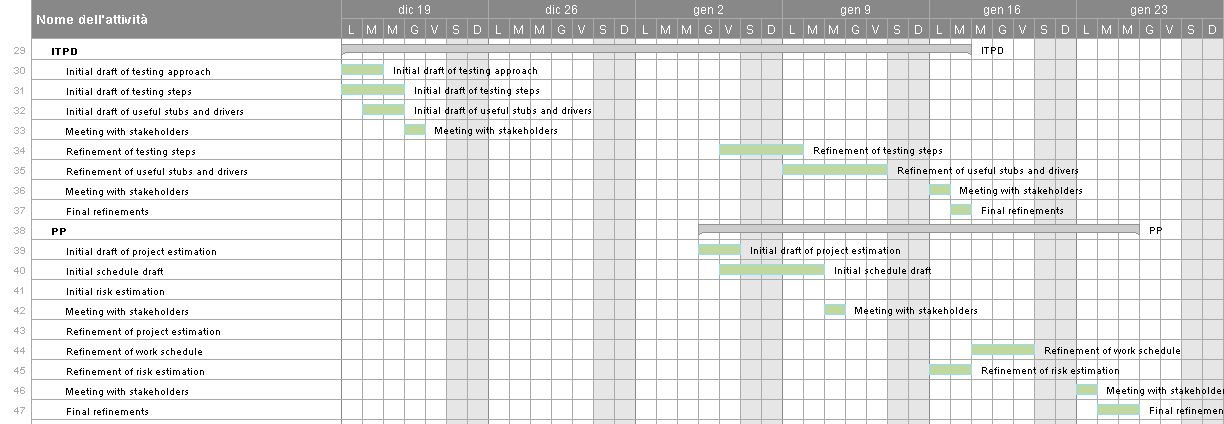
\includegraphics[width=\paperwidth]{resource_allocation/lamonaca/fl3.png}
	}
\end{center}

\begin{center}
  \makebox[\textwidth]{
    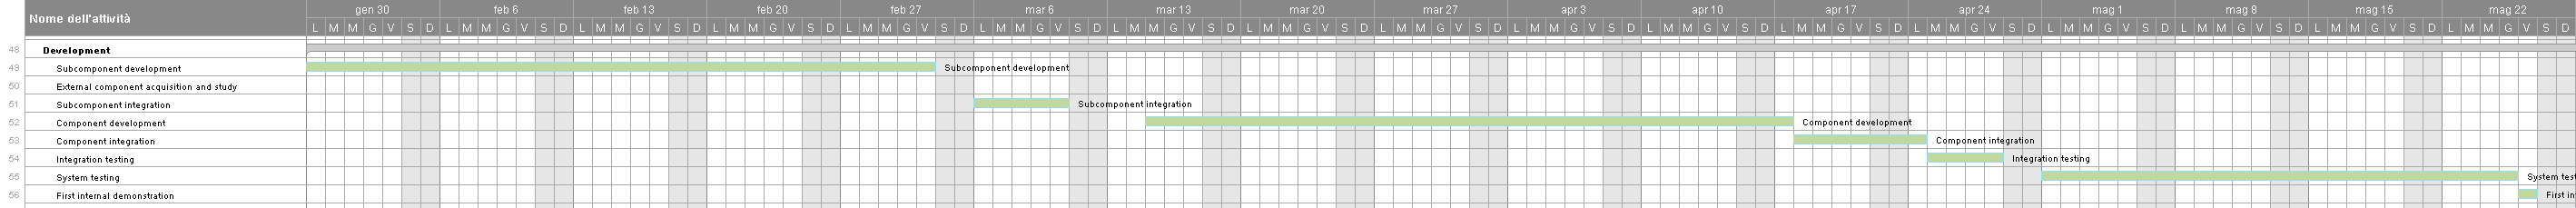
\includegraphics[width=\paperwidth]{resource_allocation/lamonaca/fl4.png}
	}
\end{center}

\begin{center}
  \makebox[\textwidth]{
    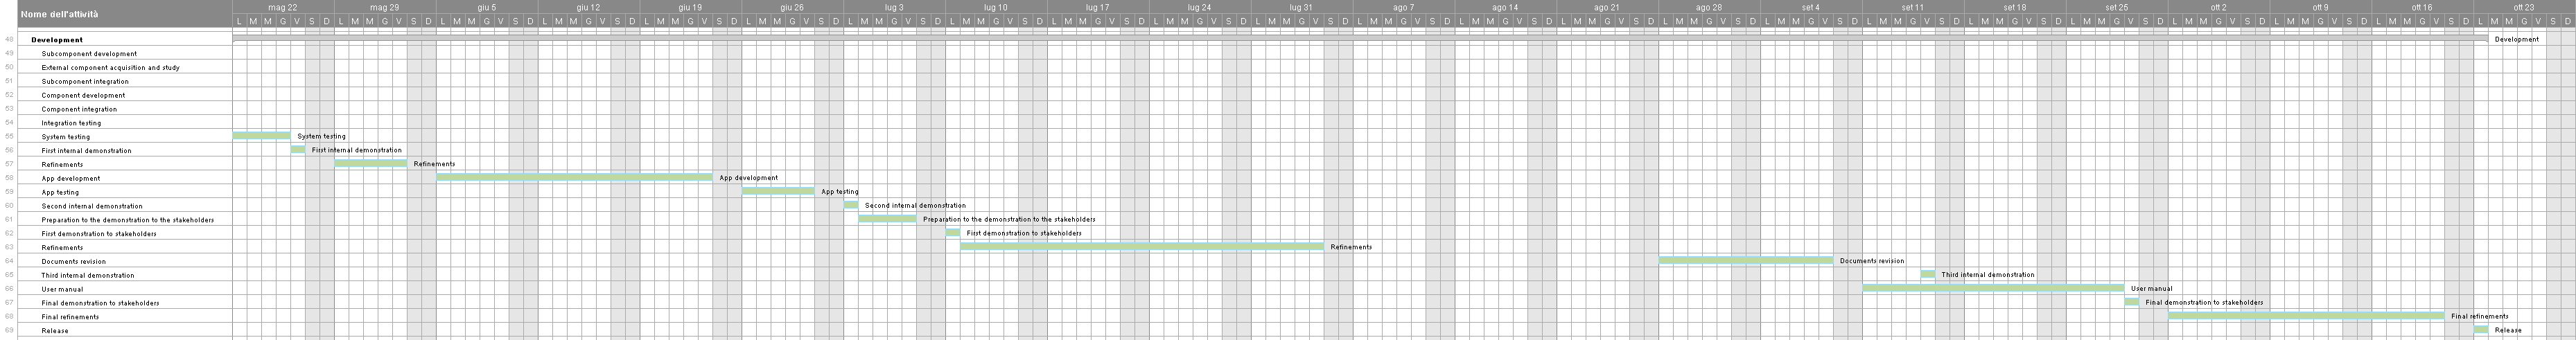
\includegraphics[width=\paperwidth]{resource_allocation/lamonaca/fl5.png}
	}
\end{center}


\section{Marco Miglionico}

\begin{center}
  \makebox[\textwidth]{
    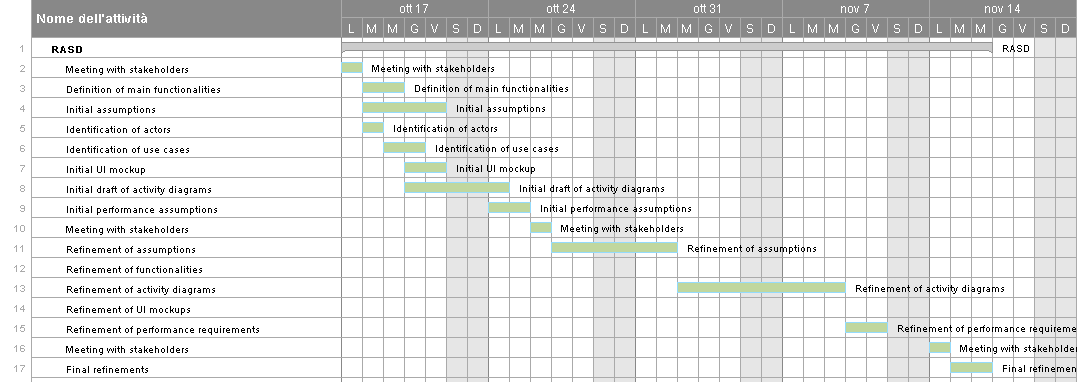
\includegraphics[width=\paperwidth]{resource_allocation/miglionico/mm1.png}
	}
\end{center}

\begin{center}
  \makebox[\textwidth]{
    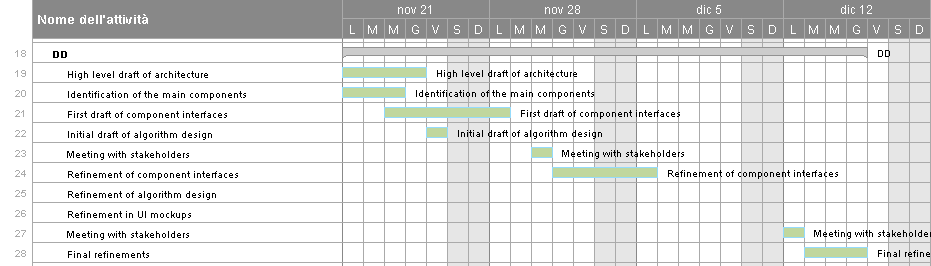
\includegraphics[width=\paperwidth]{resource_allocation/miglionico/mm2.png}
	}
\end{center}

\begin{center}
  \makebox[\textwidth]{
    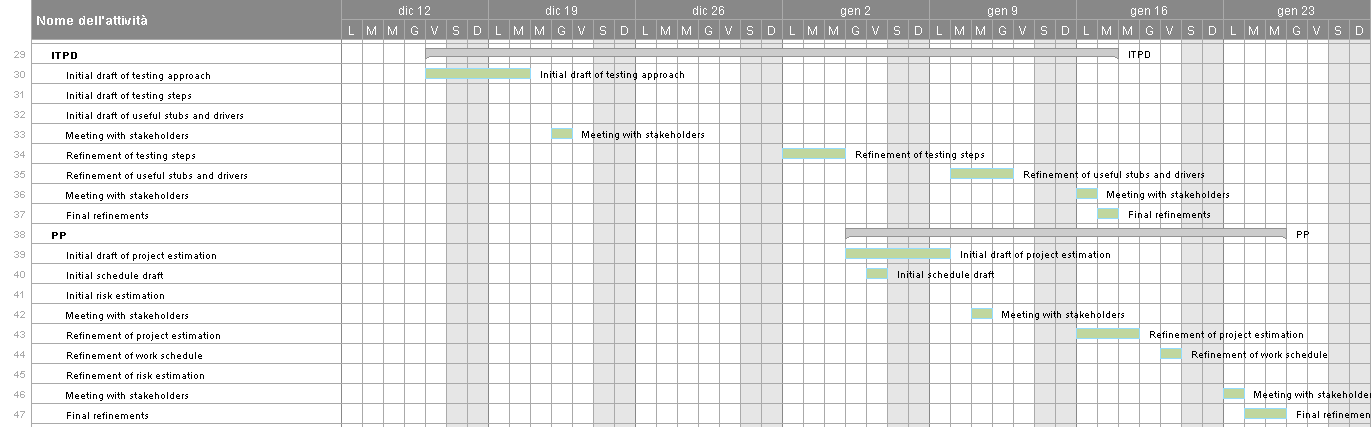
\includegraphics[width=\paperwidth]{resource_allocation/miglionico/mm3.png}
	}
\end{center}

\begin{center}
  \makebox[\textwidth]{
    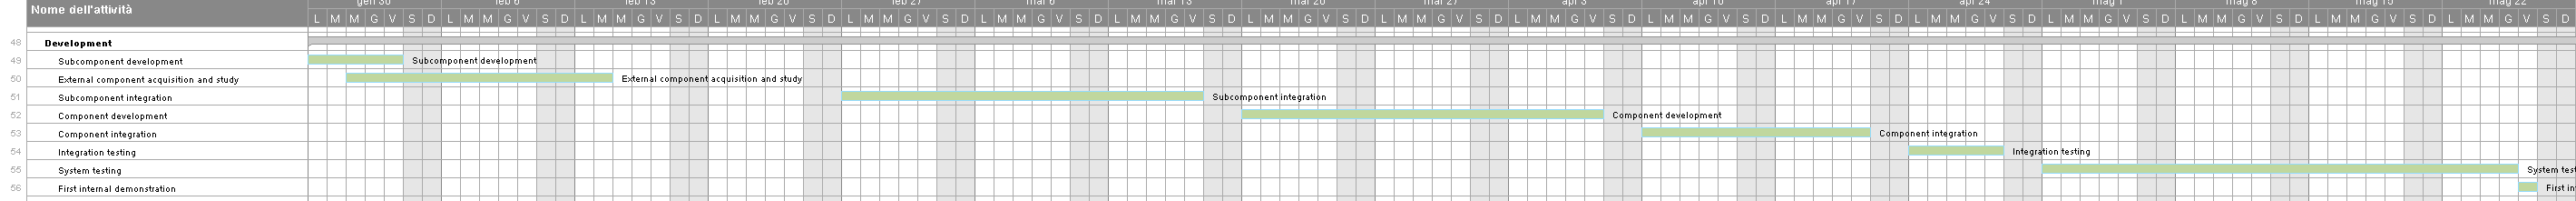
\includegraphics[width=\paperwidth]{resource_allocation/miglionico/mm4.png}
	}
\end{center}

\begin{center}
  \makebox[\textwidth]{
    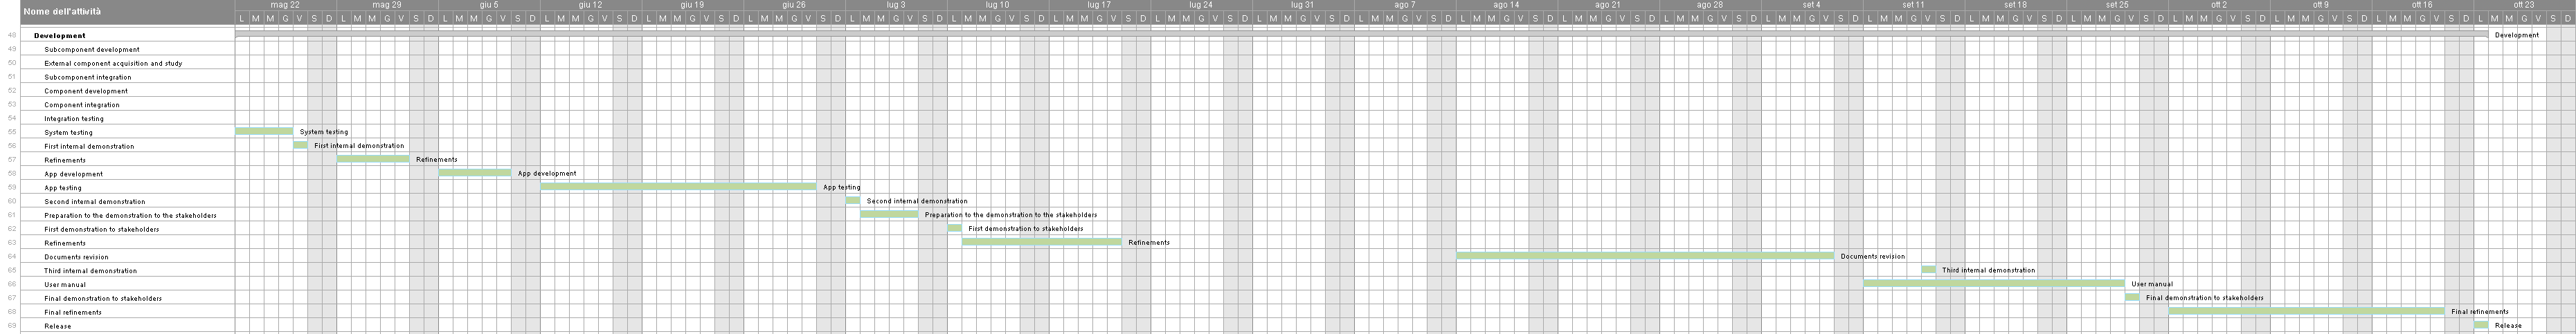
\includegraphics[width=\paperwidth]{resource_allocation/miglionico/mm5.png}
	}
\end{center}


\chapter{Risk Management}
A project development is not without any risk. In this section we will discuss some risks that our project may incur, how likely are they, what are their effects and how we would fix them. We can divide the risks into two main categories: development risk and organizational ones.
\section{Development risks}
\begin{description}
\item[Delays on the deadlines] This is the most common kind of risk during a project. However a well-defined work organization and a good parallelization of the tasks can minimize this risk. In the remote case of a delay on the final release, it may be useful to release a preliminary version of the system, with all the basic functionalities, and adding the advanced ones later.
\item[Lack of communication between members] Our group members can work from home. In this way, they can maximize the efficiency and work in an easier and more comfortable place. However the communication during the development may be more difficult but a rigorous tasks division and a well-written Project Plan may avoid some misunderstandings between members.
\item[Requirement change] Some requirements can change during development. This risk is very difficult to prevent, but writing a more flexible and modular code may reduce the effects.
\item[Code loss] Losing part or all the code is a potentially catastrophic risk. A careful back-up management may avoid this risk.
\item[Integration test failure] One or more failure during the integration test phase could create some delays one the deadlines. To minimize the effect of this risk it is needed to start the integration test phase as soon as possible.
\item[OS update incompatibility] Our application will be used on Android and iOS smartphone. In order to avoid that an update of the OS creates a conflict with our app it is needed to follow all the news made by Google and Apple for developer about further update.
\end{description}

\section{Organizational risks}
\begin{description}
\item[Car issues] Car stock is a critical resource for our system. In order to guarantee an adequate number of cars it is important to schedule a periodic maintenance.
\item[Car theft] The theft of one or more of our cars is a risk not to underestimate. Each car must be equipped with a antitheft system and a GPS to locate eventual lost cars. It is also important to insure each car.
\item[Data loss and data leak] Our system will manage some pieces of personal information, such as the payment ones. We have to protect these data to avoid a loss or a leak. Multiple back-up and adopting industry security standard can minimize this risk. 
\item[Dependency from external services] Our project will use third party services such as Google Maps or the HandyCar system. A change in the terms and conditions of one of these services may reflect on the usability of our system. A general solution for this risk does not exist, but it is our duty to contact third party to negotiate new arrangements. 
\item[Competitivity] Our service is not the first rent service to start. In order to be profitable the competitiveness of our product must be continuously enhanced by introducing innovative features and by keeping our prices competitive.
\end{description}
\appendix
\chapter{Appendix}
\section{Used software and tools}
\begin{itemize}
    \item \LaTeX\ \footnote{\url{https://www.latex-project.org/}}, for typesetting this document.
    \item Texmaker\footnote{\url{http://www.xm1math.net/texmaker/}}, for the writing of this document.
    \item GitHub\footnote{\url{https://github.com/}} for version control and distributed work.
    \item Evolus Pencil\footnote{\url{http://pencil.evolus.vn/}} for the mockups.
    \item StarUML\footnote{\url{http://staruml.io/}} for the class diagram.
    \item Alloy Analyzer\footnote{\url{http://alloy.mit.edu/alloy/}} used to build the model generated by the alloy code.
    \item Signavio Academic\footnote{\url{http://academic.signavio.com/p/login}} for the use case diagram and for BPMN.
    \item GitHub desktop\footnote{\url{https://desktop.github.com/}} used to collaborate in the team and to keep track of the changes. 
\end{itemize}

\section{Changelog}

v1.1:
\begin{itemize}
\item added car status flow chart;
\item corrected typos;
\end{itemize}

v1.0:
\begin{itemize}
\item initial release.
\end{itemize}

\section{Work hours}
The statistics about commits and code contribution are available on the GitHub repository of the project\footnote{\url{https://github.com/marcomiglionico94/Software-Engineering-2-Project}}.
Please keep in mind that some commits are the joined effort of two or all the components of the group. However, when this is the case, it is specified in the description of the commit.

These are our estimation of the work hours spent on this project:
\begin{itemize}
    \item Marco Ieni: 38 hours
    \item Francesco Lamonaca: 40 hours
    \item Marco Miglionico: 36 hours
\end{itemize}


\end{document}
